% 04-application.tex

\section{Test Application}

\begin{frame}{Secure Timeout System Application}
    \begin{itemize}
        \item The application is a simple implementation of a \textit{Secure Timeout System}.
        \item It consists of \textbf{multiple tasks} that simulate events, monitor activities, and handle alerts.
        \item \textbf{Hardware timers} are used to generate \textbf{periodic interrupts} for activity detection.
    \end{itemize}
\end{frame}

\begin{frame}{Task Implementation}
    \begin{itemize}
        \item \textbf{Event Task:}
            \begin{itemize}
                \item Periodically generates events that can be either user activities or suspicious activities.
                \item Uses a pseudo-random number generator to decide the type of event.
                \item Logs the generated event and updates the respective counters.
            \end{itemize}
    \end{itemize}
    \begin{figure}[h]
        \centering
        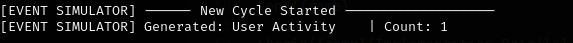
\includegraphics[width=0.75\textwidth]{images/event_task_1.png}
    \end{figure}
    \begin{figure}[h]
        \centering
        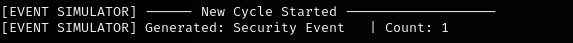
\includegraphics[width=0.75\textwidth]{images/event_task_2.png}
        \caption{Generation of a user activity and a suspicious activity.}
    \end{figure}
\end{frame}

\begin{frame}{Hardware Timer Initialization}
    \begin{itemize}
        \item \textbf{Timer 0:}
            \begin{itemize}
                \item Configured to generate periodic interrupts.
                \item Interrupt handler checks for \textbf{user activities} and sets the user activity detection flag.
            \end{itemize}
        \item \textbf{Timer 1:}
            \begin{itemize}
                \item Configured to generate periodic interrupts.
                \item Interrupt handler checks for \textbf{suspicious activities} and sets the suspicious activity detection flag.
            \end{itemize}
    \end{itemize}
\end{frame}

\begin{frame}{Task Implementation}
    \begin{itemize}
        \item \textbf{Monitor Task:}
            \begin{itemize}
                \item Checks for user activity detection.
                \item Logs the status of user activity.
                \item Resets the user activity detection flag after logging.
            \end{itemize}
        \item \textbf{Alert Task:}
            \begin{itemize}
                \item Checks for suspicious activity detection.
                \item Logs the status of the system security.
                \item Initiates security protocols if suspicious activity is detected.
                \item Resets the suspicious activity detection flag after logging.
            \end{itemize}
    \end{itemize}
\end{frame}

\begin{frame}{Implementation Details}
    \begin{itemize}
        \item \textbf{Global Variables:}
            \begin{itemize}
                \item Four main \textbf{flags}:
                    \begin{itemize}
                        \item \texttt{userActivity}, \texttt{userActivityDetection}, \\ \texttt{suspiciousActivity}, \texttt{suspiciousActivityDetection}
                    \end{itemize}
            \end{itemize}
        \item \textbf{Task Priorities:}
            \begin{itemize}
                \item Event Task has the highest priority to ensure timely event generation.
                \item Monitor Task and Alert Task have lower priorities.
            \end{itemize}
        \item \textbf{Timer Frequency:}
            \begin{itemize}
                \item Timer 0 and Timer 1 are configured to generate periodic interrupts \\at a frequency of 2 Hz.
            \end{itemize}
    \end{itemize}
\end{frame}

\begin{frame}[fragile]{Implementation Details}
    \begin{itemize}
        \item \textbf{Task Priorities:}
            \begin{lstlisting}[language=C]
// filepath: /App/SecureTimeoutSystem/secure_timeout_system.c
#define MONITOR_TASK_PRIORITY (tskIDLE_PRIORITY + 2)
#define ALERT_TASK_PRIORITY   (tskIDLE_PRIORITY + 3)
#define EVENT_TASK_PRIORITY   (tskIDLE_PRIORITY + 4)
            \end{lstlisting}
        \item \textbf{Timer Frequency:}
            \begin{lstlisting}[language=C]
// filepath: /App/Peripherals/IntTimer.c
#define tmrTIMER_0_FREQUENCY (2UL)
#define tmrTIMER_1_FREQUENCY (2UL)
            \end{lstlisting}
    \end{itemize}
\end{frame}

\begin{frame}{Run Example}
    \begin{figure}[h]
        \centering
        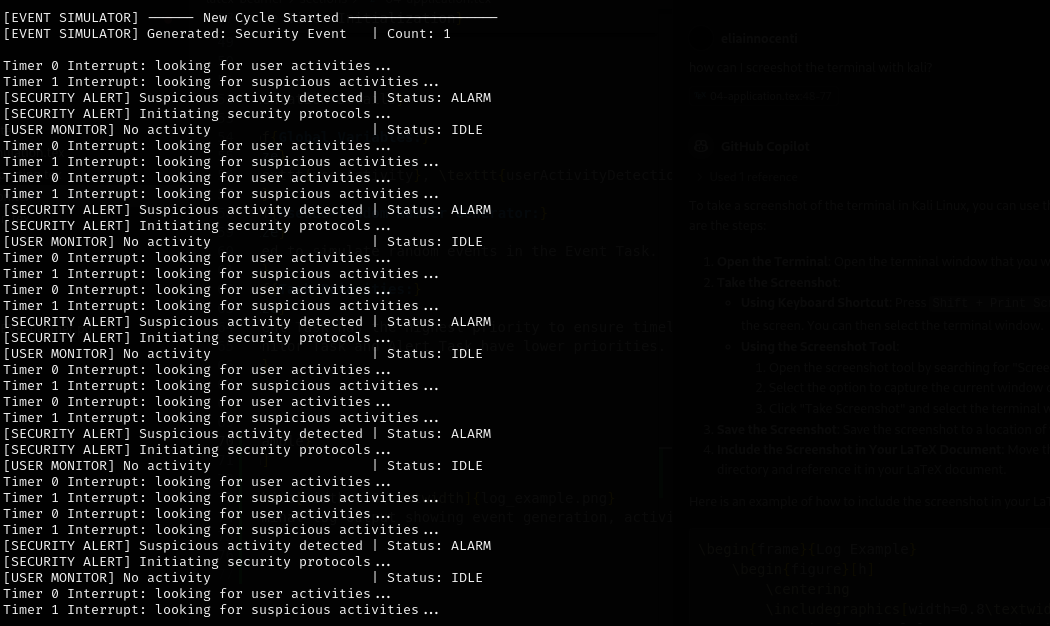
\includegraphics[width=0.75\textwidth]{images/run_example.png}
        % \caption{Terminal log output showing event generation, activity detection, and alert handling.}
    \end{figure}
\end{frame}
